\documentclass[12pt,a4paper]{article}

% Packages
\usepackage[utf8]{inputenc}
\usepackage[T1]{fontenc}
\usepackage{geometry}
\usepackage{graphicx}
\usepackage{hyperref}
\usepackage{enumitem}
\usepackage{xcolor}
\usepackage{tikz}
\usepackage{booktabs}
\usepackage{fancyhdr}
\usepackage{tcolorbox}
\usepackage{listings}
\usepackage{amsmath}
\usepackage{amssymb}
\usepackage{longtable}

% Page geometry
\geometry{margin=2.5cm}

% Colors
\definecolor{primaryblue}{RGB}{0, 102, 204}
\definecolor{successgreen}{RGB}{40, 167, 69}
\definecolor{dangerred}{RGB}{220, 53, 69}
\definecolor{warningyellow}{RGB}{255, 193, 7}
\definecolor{lightgray}{RGB}{248, 249, 250}
\definecolor{codegray}{RGB}{45, 45, 45}
\definecolor{codegreen}{RGB}{0, 128, 0}
\definecolor{purple}{RGB}{128, 0, 128}

% TikZ libraries
\usetikzlibrary{shapes, arrows, positioning, fit, backgrounds, calc}

% Listings setup
\lstset{
    basicstyle=\ttfamily\small,
    backgroundcolor=\color{lightgray},
    frame=single,
    framerule=0pt,
    breaklines=true,
    showstringspaces=false,
    keywordstyle=\color{primaryblue}\bfseries,
    commentstyle=\color{codegreen},
    stringstyle=\color{dangerred},
    numbers=left,
    numberstyle=\tiny\color{gray},
    numbersep=5pt,
    xleftmargin=15pt
}

% Header and footer
\pagestyle{fancy}
\fancyhf{}
\fancyhead[L]{\textbf{CS2113 -- Software Development Project}}
\fancyhead[R]{Lecture 3: Sprint 1}
\fancyfoot[C]{\thepage}

% Tcolorbox styles
\tcbuselibrary{skins, breakable, listings}

\newtcolorbox{keyinsight}{
    colback=primaryblue!10,
    colframe=primaryblue,
    title=\textbf{Key Insight},
    fonttitle=\bfseries,
    breakable
}

\newtcolorbox{warning}{
    colback=dangerred!10,
    colframe=dangerred,
    title=\textbf{Warning},
    fonttitle=\bfseries,
    breakable
}

\newtcolorbox{tip}{
    colback=successgreen!10,
    colframe=successgreen,
    title=\textbf{Tip},
    fonttitle=\bfseries,
    breakable
}

\newtcolorbox{definitionbox}{
    colback=lightgray,
    colframe=black!50,
    breakable
}

\newtcolorbox{commandbox}{
    colback=codegray!10,
    colframe=codegray,
    breakable
}

% Title
\title{
    \vspace{-1cm}
    \textbf{Sprint 1: Scrum and Project Setup}\\
    \large Lecture 3 Notes\\[0.5cm]
    \normalsize School of Computing Communication and Media Studies
}
\author{Masoud Hamad}
\date{CS2113 -- Software Development Project\\Academic Year 2025}

\begin{document}

\maketitle
\tableofcontents
\newpage

%============================================================
\section{Sprint Planning}
%============================================================

\begin{definitionbox}
\textbf{Sprint Planning} occurs at the beginning of each sprint with full team participation. The goal is to define what can be delivered in the upcoming Sprint and how that work will be achieved.
\end{definitionbox}

\subsection{Key Characteristics}

\begin{itemize}
    \item \textbf{Duration:} Planning typically takes a few hours maximum
    \item \textbf{Participants:} Entire Scrum Team
    \item \textbf{Output:} Sprint Backlog with selected user stories and tasks
\end{itemize}

\subsection{Roles in Sprint Planning}

\begin{itemize}
    \item \textbf{Product Owner:} Prioritizes user stories and clarifies requirements
    \item \textbf{Developers:} Provide feasibility insights and effort estimates
    \item \textbf{Scrum Master:} Facilitates the meeting and ensures process is followed
\end{itemize}

\begin{keyinsight}
Requirements tend to change during development, so Sprint Planning focuses on the near future rather than long-term projections. Plan only what you can realistically accomplish in one Sprint.
\end{keyinsight}

%------------------------------------------------------------
% Figure 1: Sprint Planning Process
%------------------------------------------------------------
\begin{figure}[htbp]
\centering
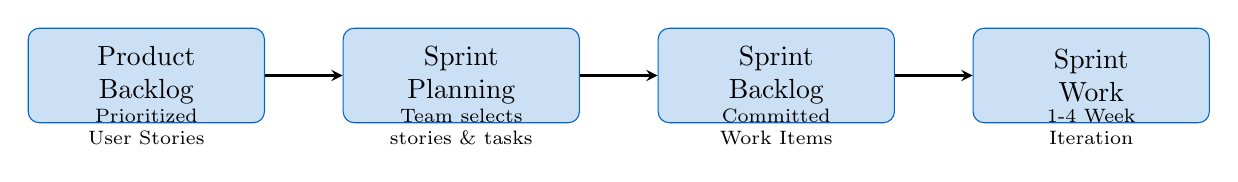
\begin{tikzpicture}[
    node distance=1cm,
    box/.style={rectangle, draw=primaryblue, fill=primaryblue!20, rounded corners, minimum width=3cm, minimum height=1.2cm, align=center},
    arrow/.style={->, thick, >=stealth}
]
    \node[box] (pb) at (0, 0) {Product\\Backlog};
    \node[box] (planning) at (4, 0) {Sprint\\Planning};
    \node[box] (sb) at (8, 0) {Sprint\\Backlog};
    \node[box] (sprint) at (12, 0) {Sprint\\Work};

    \draw[arrow] (pb) -- (planning);
    \draw[arrow] (planning) -- (sb);
    \draw[arrow] (sb) -- (sprint);

    % Labels
    \node[below=0.3cm, font=\scriptsize, align=center] at (pb) {Prioritized\\User Stories};
    \node[below=0.3cm, font=\scriptsize, align=center] at (planning) {Team selects\\stories \& tasks};
    \node[below=0.3cm, font=\scriptsize, align=center] at (sb) {Committed\\Work Items};
    \node[below=0.3cm, font=\scriptsize, align=center] at (sprint) {1-4 Week\\Iteration};
\end{tikzpicture}
\caption{Sprint Planning Flow}
\label{fig:sprint-planning}
\end{figure}

%============================================================
\section{User Stories and Tasks}
%============================================================

\subsection{From User Stories to Tasks}

User stories are written from the user's perspective \textbf{without technical details}. During Sprint Planning, developers split each story into \textbf{technical tasks} containing specific implementation requirements.

\begin{definitionbox}
\textbf{Tasks} are small, technical work items derived from user stories. Each task should be completable in a few hours to a day.
\end{definitionbox}

\subsection{Example: Breaking Down a User Story}

\textbf{User Story:} ``As a content creator, I want to create a blog so I can write posts for readers.''

\textbf{Technical Tasks:}
\begin{enumerate}
    \item Create UI form with text fields and submit button
    \item Create Blog entity class with JPA annotations
    \item Create BlogRepository interface
    \item Create BlogController with POST endpoint
    \item Configure H2 database connection
    \item Write unit tests for BlogService
\end{enumerate}

%------------------------------------------------------------
% Figure 2: User Story to Tasks
%------------------------------------------------------------
\begin{figure}[htbp]
\centering
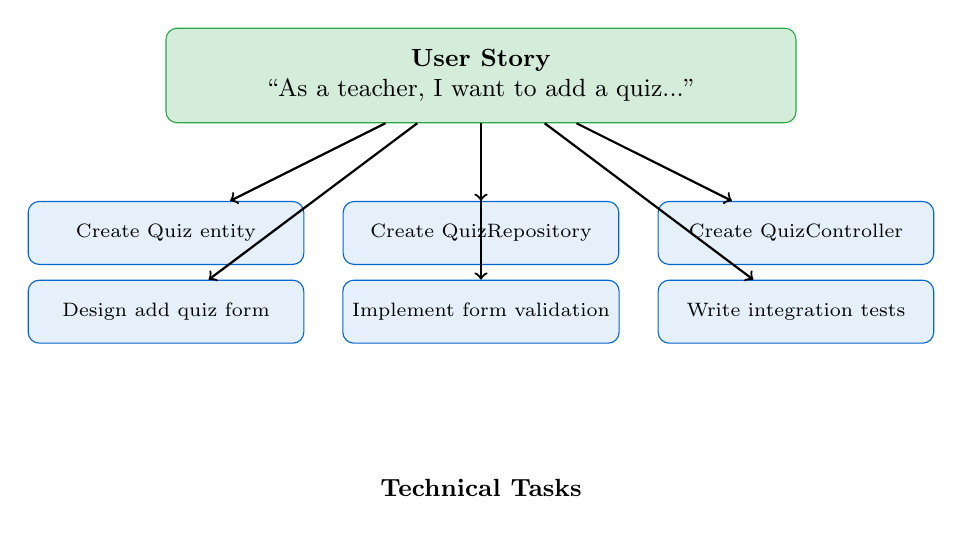
\begin{tikzpicture}[
    node distance=0.8cm,
    story/.style={rectangle, draw=successgreen, fill=successgreen!20, rounded corners, minimum width=8cm, minimum height=1.2cm, align=center, font=\small},
    task/.style={rectangle, draw=primaryblue, fill=primaryblue!10, rounded corners, minimum width=3.5cm, minimum height=0.8cm, align=center, font=\scriptsize},
    arrow/.style={->, thick}
]
    \node[story] (story) at (0, 3) {\textbf{User Story}\\``As a teacher, I want to add a quiz...''};

    \node[task] (t1) at (-4, 1) {Create Quiz entity};
    \node[task] (t2) at (0, 1) {Create QuizRepository};
    \node[task] (t3) at (4, 1) {Create QuizController};
    \node[task] (t4) at (-4, 0) {Design add quiz form};
    \node[task] (t5) at (0, 0) {Implement form validation};
    \node[task] (t6) at (4, 0) {Write integration tests};

    \draw[arrow] (story) -- (t1);
    \draw[arrow] (story) -- (t2);
    \draw[arrow] (story) -- (t3);
    \draw[arrow] (story) -- (t4);
    \draw[arrow] (story) -- (t5);
    \draw[arrow] (story) -- (t6);

    \node[below=1.5cm, font=\small\bfseries] at (0, -0.5) {Technical Tasks};
\end{tikzpicture}
\caption{Breaking User Stories into Technical Tasks}
\label{fig:story-to-tasks}
\end{figure}

%============================================================
\section{Scrum Backlogs}
%============================================================

\subsection{Product Backlog}

\begin{definitionbox}
The \textbf{Product Backlog} is a prioritized list of all requirements (primarily user stories) for the product. The Product Owner maintains priorities; highest-priority items appear first.
\end{definitionbox}

\textbf{Characteristics:}
\begin{itemize}
    \item Contains all user stories for the entire project
    \item Ordered by priority (most important at top)
    \item Items are removed once implemented and accepted
    \item Continuously refined and updated
\end{itemize}

\subsection{Sprint Backlog}

\begin{definitionbox}
The \textbf{Sprint Backlog} contains the technical tasks selected from the Product Backlog for the current Sprint. It tracks task progress throughout the Sprint.
\end{definitionbox}

\textbf{Sprint Backlog tracks:}
\begin{itemize}
    \item Which user story each task relates to
    \item Team member assignments
    \item Task progress (Not Started, In Progress, Done)
\end{itemize}

%------------------------------------------------------------
% Figure 3: Product Backlog vs Sprint Backlog
%------------------------------------------------------------
\begin{figure}[htbp]
\centering
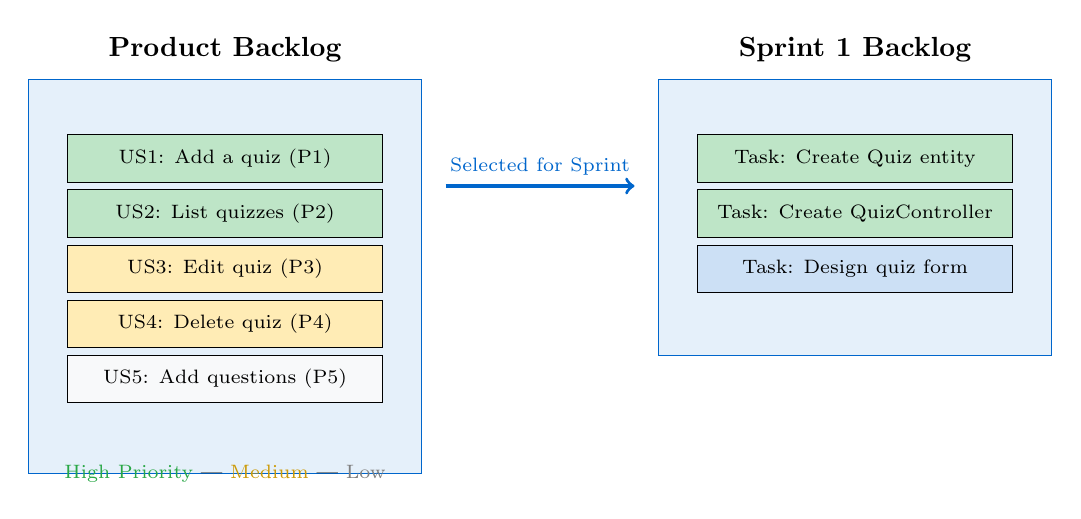
\begin{tikzpicture}[
    node distance=0.5cm,
    item/.style={rectangle, draw, fill=white, minimum width=4cm, minimum height=0.6cm, font=\scriptsize},
    backlog/.style={rectangle, draw=primaryblue, fill=primaryblue!10, minimum width=5cm, minimum height=5cm}
]
    % Product Backlog
    \node[backlog] (pb) at (0, 0) {};
    \node[above=0.1cm, font=\bfseries] at (pb.north) {Product Backlog};

    \node[item, fill=successgreen!30] at (0, 1.5) {US1: Add a quiz (P1)};
    \node[item, fill=successgreen!30] at (0, 0.8) {US2: List quizzes (P2)};
    \node[item, fill=warningyellow!30] at (0, 0.1) {US3: Edit quiz (P3)};
    \node[item, fill=warningyellow!30] at (0, -0.6) {US4: Delete quiz (P4)};
    \node[item, fill=lightgray] at (0, -1.3) {US5: Add questions (P5)};

    % Sprint Backlog
    \node[backlog, minimum height=3.5cm] (sb) at (8, 0.75) {};
    \node[above=0.1cm, font=\bfseries] at (sb.north) {Sprint 1 Backlog};

    \node[item, fill=successgreen!30] at (8, 1.5) {Task: Create Quiz entity};
    \node[item, fill=successgreen!30] at (8, 0.8) {Task: Create QuizController};
    \node[item, fill=primaryblue!20] at (8, 0.1) {Task: Design quiz form};

    % Arrow
    \draw[->, very thick, primaryblue] (2.8, 1.15) -- node[above, font=\scriptsize] {Selected for Sprint} (5.2, 1.15);

    % Legend
    \node[font=\scriptsize] at (0, -2.5) {\textcolor{successgreen}{High Priority} | \textcolor{warningyellow!80!black}{Medium} | \textcolor{gray}{Low}};
\end{tikzpicture}
\caption{Product Backlog vs Sprint Backlog}
\label{fig:backlogs}
\end{figure}

%============================================================
\section{Task Board and GitHub Projects}
%============================================================

\subsection{Virtual Task Boards}

A task board visualizes work progress using columns representing different states:

\begin{center}
\begin{tabular}{|c|c|c|c|}
\hline
\textbf{Product Backlog} & \textbf{Sprint Backlog} & \textbf{In Progress} & \textbf{Done} \\
\hline
Future items & Committed work & Currently working & Completed \\
\hline
\end{tabular}
\end{center}

\subsection{GitHub Projects Setup}

\begin{enumerate}
    \item Navigate to your repository on GitHub
    \item Click ``Projects'' tab
    \item Create a new project named ``Backlog''
    \item Add columns: Product Backlog, Sprint Backlog, In Progress, Done
    \item Make the project public
\end{enumerate}

%------------------------------------------------------------
% Figure 4: Kanban Board
%------------------------------------------------------------
\begin{figure}[htbp]
\centering
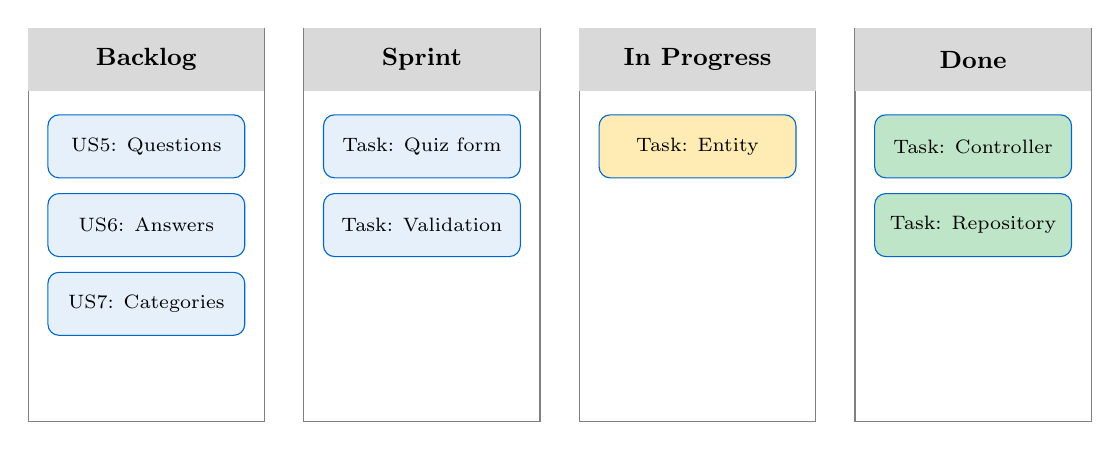
\begin{tikzpicture}[
    column/.style={rectangle, draw=gray, minimum width=3cm, minimum height=5cm},
    card/.style={rectangle, draw=primaryblue, fill=primaryblue!10, rounded corners, minimum width=2.5cm, minimum height=0.8cm, font=\scriptsize, align=center},
    header/.style={rectangle, fill=gray!30, minimum width=3cm, minimum height=0.8cm, font=\small\bfseries}
]
    % Columns
    \node[column] (c1) at (0, 0) {};
    \node[column] (c2) at (3.5, 0) {};
    \node[column] (c3) at (7, 0) {};
    \node[column] (c4) at (10.5, 0) {};

    % Headers
    \node[header] at (0, 2.1) {Backlog};
    \node[header] at (3.5, 2.1) {Sprint};
    \node[header] at (7, 2.1) {In Progress};
    \node[header] at (10.5, 2.1) {Done};

    % Cards
    \node[card] at (0, 1) {US5: Questions};
    \node[card] at (0, 0) {US6: Answers};
    \node[card] at (0, -1) {US7: Categories};

    \node[card] at (3.5, 1) {Task: Quiz form};
    \node[card] at (3.5, 0) {Task: Validation};

    \node[card, fill=warningyellow!30] at (7, 1) {Task: Entity};

    \node[card, fill=successgreen!30] at (10.5, 1) {Task: Controller};
    \node[card, fill=successgreen!30] at (10.5, 0) {Task: Repository};
\end{tikzpicture}
\caption{Kanban-style Task Board}
\label{fig:kanban}
\end{figure}

%============================================================
\section{GitHub Issues and Milestones}
%============================================================

\subsection{Creating Labels}

Labels help categorize issues:
\begin{itemize}
    \item \texttt{user story} -- For user story issues
    \item \texttt{bug} -- For bug reports
    \item \texttt{frontend} -- For frontend tasks
    \item \texttt{backend} -- For backend tasks
\end{itemize}

\subsection{Creating Milestones}

Milestones group issues for a specific Sprint:
\begin{enumerate}
    \item Go to Issues $\rightarrow$ Milestones
    \item Create ``Sprint 1'' milestone
    \item Set a due date (end of Sprint)
\end{enumerate}

\subsection{Creating Issues}

For each user story and task:
\begin{enumerate}
    \item Set descriptive title
    \item Add appropriate label(s)
    \item Assign to team member
    \item Set milestone (Sprint 1, 2, or 3)
    \item Add to Backlog project
\end{enumerate}

%============================================================
\section{Daily Scrum}
%============================================================

\begin{definitionbox}
The \textbf{Daily Scrum} is a 15-minute daily event where team members synchronize activities and create a plan for the next 24 hours.
\end{definitionbox}

\subsection{Three Questions}

Each team member answers:
\begin{enumerate}
    \item What did I complete since the last meeting?
    \item What will I work on next?
    \item Are there any obstacles blocking my progress?
\end{enumerate}

\begin{tip}
The Daily Scrum is often called ``daily stand-up'' because standing discourages lengthy discussions. Keep it short and focused!
\end{tip}

%------------------------------------------------------------
% Figure 5: Daily Scrum
%------------------------------------------------------------
\begin{figure}[htbp]
\centering
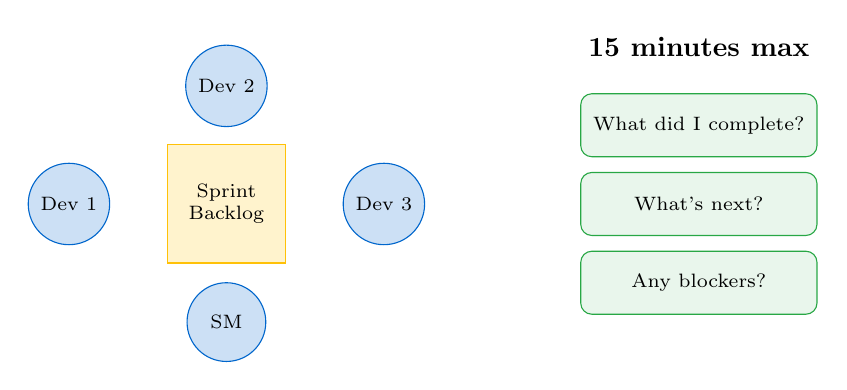
\begin{tikzpicture}[
    person/.style={circle, draw=primaryblue, fill=primaryblue!20, minimum size=1cm, font=\scriptsize},
    question/.style={rectangle, draw=successgreen, fill=successgreen!10, rounded corners, minimum width=3cm, minimum height=0.8cm, font=\scriptsize, align=center}
]
    % Team members
    \node[person] (p1) at (0, 0) {Dev 1};
    \node[person] (p2) at (2, 1.5) {Dev 2};
    \node[person] (p3) at (4, 0) {Dev 3};
    \node[person] (p4) at (2, -1.5) {SM};

    % Center - Sprint Backlog
    \node[rectangle, draw=warningyellow, fill=warningyellow!20, minimum width=1.5cm, minimum height=1.5cm, font=\scriptsize, align=center] at (2, 0) {Sprint\\Backlog};

    % Questions
    \node[question] at (8, 1) {What did I complete?};
    \node[question] at (8, 0) {What's next?};
    \node[question] at (8, -1) {Any blockers?};

    % Time
    \node[font=\bfseries] at (8, 2) {15 minutes max};
\end{tikzpicture}
\caption{Daily Scrum Meeting Structure}
\label{fig:daily-scrum}
\end{figure}

%============================================================
\section{Teamwork Best Practices}
%============================================================

\begin{itemize}
    \item Work collaboratively and divide tasks deliberately
    \item Maintain active communication about progress
    \item Push code frequently: \texttt{git add}, \texttt{git commit}, \texttt{git push}
    \item Pull frequently: \texttt{git pull}
    \item Expect and handle merge conflicts
    \item Adjust Sprint Backlog as needed during implementation
\end{itemize}

\begin{warning}
Tasks aren't immutable! If you discover a task is more complex than expected, discuss with your team and adjust the Sprint Backlog accordingly.
\end{warning}

%============================================================
\section{REST API Basics}
%============================================================

\subsection{Introduction to REST Controllers}

For the frontend to access backend data, we create REST API endpoints:

\begin{commandbox}
\begin{lstlisting}[language=Java]
@RestController
@RequestMapping("/api")
@CrossOrigin(origins = "*")
public class QuizRestController {

    @Autowired
    private QuizRepository quizRepository;

    @GetMapping("/quizzes")
    public List<Quiz> getPublishedQuizzes() {
        return quizRepository.findByPublishedTrue();
    }
}
\end{lstlisting}
\end{commandbox}

\subsection{CORS (Cross-Origin Resource Sharing)}

The frontend (Vite on port 5173) and backend (Spring Boot on port 8080) run on different origins. The \texttt{@CrossOrigin} annotation enables cross-origin requests.

\subsection{Fetching Data in Frontend}

\begin{commandbox}
\begin{lstlisting}[language=JavaScript]
fetch("http://localhost:8080/api/quizzes")
    .then(response => response.json())
    .then(quizzes => {
        console.log(quizzes);
    });
\end{lstlisting}
\end{commandbox}

%============================================================
\section{Developer Guide Documentation}
%============================================================

The README.md should include clear instructions for starting the application:

\begin{commandbox}
\begin{lstlisting}[language=markdown]
## Developer Guide

### Prerequisites
- Java 21 or higher
- Maven

### Running the Backend
1. Clone the repository
2. Navigate to project folder
3. Run: ./mvnw spring-boot:run
4. Access: http://localhost:8080
\end{lstlisting}
\end{commandbox}

\begin{tip}
Test your developer guide by having a team member follow the instructions exactly on a fresh clone of the repository!
\end{tip}

%============================================================
\section{GitHub Releases}
%============================================================

Releases ``freeze'' source code at specific commit points:

\begin{enumerate}
    \item Go to repository $\rightarrow$ Releases
    \item Click ``Create a new release''
    \item Create tag (e.g., \texttt{sprint1})
    \item Set title (e.g., ``Sprint 1'')
    \item Describe implemented features
    \item Publish release
\end{enumerate}

%============================================================
\section{Sprint Review}
%============================================================

\begin{definitionbox}
The \textbf{Sprint Review} occurs at the end of each Sprint. The team demonstrates implemented user stories to the Product Owner and stakeholders.
\end{definitionbox}

\subsection{Sprint Review Requirements}

\begin{itemize}
    \item Working application (ideally deployed)
    \item Sensible test data (no ``test123'' placeholders)
    \item Clear demonstration of features from \textbf{user perspective}
    \item Focus on functionality, not code
\end{itemize}

%============================================================
\newpage
\section{Exercises}
%============================================================

\begin{tcolorbox}[colback=warningyellow!10, colframe=warningyellow!80!black, title=\textbf{Sprint 1 Deadline}]
All work must be pushed to GitHub repository before the Sprint deadline.
\end{tcolorbox}

\subsection{Exercise 1: Create Backlog Project}
Create a GitHub Project named ``Backlog'' with columns: Product Backlog, Sprint Backlog, In Progress, Done.

\subsection{Exercise 2: Select Scrum Master}
Choose a Scrum Master for Sprint 1 from your team.

\subsection{Exercise 3: Create Labels}
Create a ``user story'' label in your repository for categorizing user story issues.

\subsection{Exercise 4: Create Milestone}
Create a ``Sprint 1'' milestone to group Sprint-related issues.

\subsection{Exercise 5: Create User Story Issues}
Create GitHub issues for each Sprint 1 user story with appropriate labels and milestone.

\subsection{Exercise 6: Database Planning}
Plan your database schema:
\begin{itemize}
    \item Identify required entities
    \item Define entity attributes
    \item Determine relationships
    \item Configure H2 database in \texttt{application.properties}
\end{itemize}

\subsection{Exercises 7--10: Task Planning}
For each user story (Add Quiz, List Quizzes, Edit Quiz, Delete Quiz):
\begin{itemize}
    \item Break down into technical tasks
    \item Create issues for each task
    \item Assign team members
    \item Add to Sprint Backlog
\end{itemize}

\subsection{Exercise 11: Assign Team Members}
Assign team members to all task issues based on skills and workload balance.

\subsection{Exercise 12: Daily Scrum}
Conduct Daily Scrum meetings throughout the Sprint, answering the three questions.

\subsection{Exercises 13--18: Additional Task Planning}
Plan tasks for remaining user stories (Questions, Answer Options management).

\subsection{Exercise 19: Initialize Frontend}
Create a frontend application (using Vite/React) in your repository.

\subsection{Exercise 20: REST Controller}
Implement a REST controller method returning only published quizzes.

\subsection{Exercise 21: Frontend Quiz List}
Implement quiz listing on the student frontend using fetch API.

\subsection{Exercise 22: Developer Guide}
Write a developer guide in README.md with backend startup instructions.

\subsection{Exercise 23: Deploy Backend}
Deploy your backend application to the production environment.

\subsection{Exercise 24: Create Release}
Create a GitHub release named ``Sprint 1'' with implemented features description.

\subsection{Exercise 25: Sprint Review Preparation}
Prepare demonstration for Sprint Review:
\begin{itemize}
    \item Ensure working application
    \item Prepare test data
    \item Practice demo from user perspective
\end{itemize}

%============================================================
\section*{Bonus: Feature Branch Workflow}
%============================================================

\begin{commandbox}
\begin{lstlisting}[language=bash]
# Create and switch to feature branch
git checkout -b feature/add-quiz

# Work on feature...
git add .
git commit -m "Implement add quiz feature"

# Push branch to remote
git push --set-upstream origin feature/add-quiz

# Create Pull Request on GitHub
# After review, merge to main
\end{lstlisting}
\end{commandbox}

%============================================================
\vspace{1cm}
\hrule
\vspace{0.3cm}
\begin{center}
\small
\textit{This document is licensed under Creative Commons BY-NC-SA 4.0}
\end{center}

\end{document}
